\documentclass[11pt,a4paper]{article}
\usepackage[T1]{fontenc}
\usepackage[utf8]{inputenc}
\usepackage{libertinus}
\usepackage[scaled=0.92]{sourcesanspro}
\usepackage[margin=2.5cm,top=2.4cm,bottom=2.6cm]{geometry}
\usepackage{microtype,booktabs,graphicx,amsmath,enumitem,xcolor,caption,tabularx}
\usepackage[most]{tcolorbox}
\usepackage{titlesec}
\usepackage[authoryear,round]{natbib}
\usepackage[hidelinks]{hyperref}
\usepackage{fancyhdr}

\definecolor{navy}{RGB}{31,58,95}
\definecolor{band}{RGB}{242,245,249}
\definecolor{accent}{RGB}{200,135,58}
\hypersetup{colorlinks=true,linkcolor=navy,citecolor=navy,urlcolor=navy}

\titleformat{\section}{\sffamily\Large\bfseries\color{navy}}{\thesection}{0.8em}{}
\titleformat{\subsection}{\sffamily\large\bfseries\color{navy}}{\thesubsection}{0.7em}{}
\titleformat{\paragraph}[runin]{\sffamily\bfseries}{}{}{}[.]
\titlespacing*{\section}{0pt}{1.6em}{0.6em}
\titlespacing*{\subsection}{0pt}{1.2em}{0.4em}
\captionsetup{font=small,labelfont={bf,sf,color=navy},labelsep=period,justification=raggedright,singlelinecheck=false}
\setlist{itemsep=0.25em,topsep=0.4em}
\setlength{\parskip}{0.45em}
\setlength{\parindent}{0pt}
\linespread{1.08}

\pagestyle{fancy}\fancyhf{}
\renewcommand{\headrulewidth}{0pt}
\fancyfoot[L]{\small\sffamily\color{gray}P. Gaspar --- PPO exposure agent on the SMI: an audit}
\fancyfoot[R]{\small\sffamily\color{gray}\thepage}

\newtcolorbox{keybox}[1][]{colback=band,colframe=navy,boxrule=0pt,leftrule=3pt,arc=0pt,
  left=10pt,right=10pt,top=7pt,bottom=7pt,fonttitle=\sffamily\bfseries\color{navy},
  coltitle=navy,colbacktitle=band,title={#1},attach title to upper,after title={\par\smallskip}}

\newcommand{\pct}[1]{#1\%}

\begin{document}

% ------------------------------------------------------------------ title
\begin{titlepage}
\vspace*{2.5cm}
{\sffamily\small\color{accent}\bfseries REVISED PORTFOLIO EDITION OF AN MSC THESIS}\par\vspace{0.8em}
{\sffamily\fontsize{24}{29}\selectfont\bfseries\color{navy} Learned Timing or\\Cost-Induced Cash?\par}
\vspace{0.6em}
{\sffamily\Large A reproducibility audit of a PPO exposure agent\\on the Swiss Market Index\par}
\vspace{2.2cm}
{\large Pedro Gabriel Silva Gaspar\par}
\vspace{0.3em}
{\small MSc in Data Science and Advanced Analytics (Business Analytics)\\
NOVA Information Management School, Universidade Nova de Lisboa\par}
\vspace{2.2cm}
\begin{keybox}[About this edition]
\small
This document is a rewritten, extended edition of my MSc thesis \emph{Dynamic Exposure Management and Downside Risk Mitigation in the Swiss Market: A Deep Reinforcement Learning Approach} (supervisor: Prof.\ João Martins), defended on 28 October 2026.

It differs from the thesis in three ways. (1)~It corrects how the reported model was trained: the saved model behind the thesis's main table was trained for about 1,000,000 timesteps on the full 2010--2024 series, so its test-period results are in-sample, not out-of-sample as the thesis stated. (2)~It adds the analyses I ran after submission: an out-of-sample control, 30 seeded re-trainings, consistent cash accounting, formal Sharpe-ratio tests, a turnover-cost agent and stress windows. (3)~It reframes the conclusions to match that evidence.
\end{keybox}
\vfill
{\small\color{gray} November 2026}
\end{titlepage}

% ------------------------------------------------------------------ abstract
\begin{abstract}
\noindent
Deep reinforcement learning (DRL) papers on trading often report high Sharpe ratios on a single back-test. This study takes one such result, my own, and audits it. A Proximal Policy Optimization (PPO) agent chooses each day how much of its capital to hold in the Swiss Market Index (SMI), from 0\% to 100\%, using the index level, the RSI and the MACD as its state. On 2023--2024 the reported agent had a Sharpe ratio of 1.17 and a maximum drawdown of $-0.77\%$, against 0.30 and $-10.97\%$ for buy-and-hold.

The audit finds four things. First, the reported model was trained on data that included the test years. A control trained only on 2010--2022 (three seeds) gives the same picture out-of-sample (Sharpe 1.04--1.29, drawdown $-0.62\%$ to $-1.08\%$), so the leak did not create the result, but it did not validate it either. Second, the reward charges 0.1\% per day on the exposure held, about five times the SMI's average daily return, so the agent sits in cash: it was invested on 27 of 499 test days. The low drawdown is mostly a consequence of not being in the market. Third, under consistent accounting (idle cash earns SARON, every strategy pays the same trading cost) the agent returns 7.5\% against 14.3\% for total-return buy-and-hold and 15.3\% for a real 60/40 portfolio, and no Sharpe-ratio difference is significant at 5\% (studentized block-bootstrap tests, $p=0.26$ to $0.77$). Fourth, an agent redesigned with a turnover cost does take real exposure, but its edge over simple rules is not significant and disappears at a cost of 0.25\% per trade. In two stress windows (2020 and 2022) neither agent showed learned de-risking.

The contribution is therefore methodological: a worked example of how a promising DRL back-test can be explained by its cost specification and its accounting, and a checklist for testing such claims.

\medskip
\noindent\textbf{Keywords:} deep reinforcement learning; PPO; market timing; Swiss Market Index; back-test overfitting; Sharpe-ratio testing; reproducibility.
\end{abstract}

\begin{keybox}[Findings at a glance]
\small
\begin{tabularx}{\linewidth}{@{}p{4.6cm}X@{}}
\textbf{What the thesis reported} & Sharpe 1.17 vs 0.30 for buy-and-hold; drawdown $-0.77\%$ vs $-10.97\%$ (2023--2024). \\[2pt]
\textbf{How the model was trained} & 1,001,472 timesteps on 2010--2024, test years included (not 10,000 timesteps on 2010--2022). \\[2pt]
\textbf{Out-of-sample control} & Trained on 2010--2022 only, 3 seeds: same behaviour, Sharpe 1.04--1.29. \\[2pt]
\textbf{Why the drawdown is low} & A 0.1\%/day holding cost $\approx$ 5$\times$ the mean daily return; the agent is invested 27 of 499 days. \\[2pt]
\textbf{Fair comparison} & 7.5\% vs 14.3\% (buy-and-hold with dividends) and 15.3\% (real 60/40). \\[2pt]
\textbf{Statistical tests} & No Sharpe difference significant at 5\% ($p = 0.26$--$0.77$). \\[2pt]
\textbf{Redesigned agent} & Takes real exposure; no significant edge; gone at 0.25\% per trade. \\
\end{tabularx}
\end{keybox}

\newpage
\tableofcontents
\newpage

% ------------------------------------------------------------------ 1
\section{Introduction}

Static allocations such as buy-and-hold or a 60/40 equity--bond mix keep the same exposure in every market regime, so they take the full drawdown when markets fall. A natural question is whether a learning agent can do better by adjusting its exposure to market conditions. Deep reinforcement learning (DRL) is a popular tool for this: the agent observes a state, chooses an action, receives a reward and learns a policy by trial and error \citep{jiang2017,xiong2018,yang2020}.

Most published DRL trading studies focus on U.S.\ equities or cryptocurrencies, and they usually report one back-test of one trained model. The Swiss market has received little attention, although it differs from the U.S.\ in ways that matter for a timing agent: the SMI is concentrated in a few defensive large caps, Swiss interest rates were negative until 2022, and Swiss trades pay a federal stamp duty.

My MSc thesis trained a PPO agent \citep{schulman2017} to set its daily exposure to the SMI between 0\% and 100\%. On 2023--2024 it reported a Sharpe ratio almost four times that of buy-and-hold, with a maximum drawdown close to zero. This edition asks a stricter question: \emph{does that result show learned market timing, or can it be explained by the design of the experiment?}

\paragraph{Contributions}
\begin{enumerate}[leftmargin=1.4em]
  \item \textbf{A provenance audit} of the reported model. Its saved file shows that it was trained on the test years. I document this and replace the in-sample claim with an out-of-sample control (Section~\ref{sec:provenance}).
  \item \textbf{A decomposition of the headline result.} I show that the cost specification makes cash the near-optimal action, and that fair cash accounting reverses the ranking against real benchmarks (Sections~\ref{sec:cash}--\ref{sec:fair}).
  \item \textbf{Formal inference} on Sharpe ratios with a studentized circular block bootstrap \citep{ledoit2008} and Holm adjustment \citep{holm1979}, across 30 + 10 + 6 trained agents (Section~\ref{sec:tests}).
  \item \textbf{A corrected agent and stress tests}, which show what changes when the cost is charged on trading instead of holding (Sections~\ref{sec:turnover}--\ref{sec:stress}).
\end{enumerate}

\paragraph{Hypotheses} The thesis stated two hypotheses, kept here so that they can be closed honestly in Section~\ref{sec:discussion}.
\textbf{H1}: the PPO agent achieves a higher Sharpe ratio than SMI buy-and-hold on the test period.
\textbf{H2}: the PPO agent achieves a smaller maximum drawdown than both buy-and-hold and a static 60/40 portfolio on the test period.

% ------------------------------------------------------------------ 2
\section{Related work}

\paragraph{DRL for allocation and trading} \citet{jiang2017} introduced an end-to-end DRL framework for portfolio management on cryptocurrency pairs. \citet{xiong2018} and \citet{yang2020} applied DDPG and an ensemble of PPO, A2C and DDPG to the 30 Dow Jones stocks, reporting Sharpe ratios above the index. Later work extended the setting to other markets and objectives: \citet{hieu2020} on U.S.\ stock pools, \citet{garrido2023} on ESG-aware portfolios in the DJIA, IBEX~35 and NASDAQ-100, \citet{wu2024} on the Australian ASX50, and \citet{hirsa2021} on E-mini S\&P~500 futures. Table~\ref{tab:lit} summarises them. None of them studies the Swiss market, and most evaluate one trained model on one test window.

\begin{table}[ht]
\centering\small
\caption{Prior DRL studies on allocation and trading, and the position of this study.}
\label{tab:lit}
\begin{tabularx}{\linewidth}{@{}>{\raggedright\arraybackslash}p{3.6cm}>{\raggedright\arraybackslash}X>{\raggedright\arraybackslash}p{3.0cm}c@{}}
\toprule
\textbf{Study} & \textbf{Market} & \textbf{Universe} & \textbf{Swiss} \\
\midrule
\citet{jiang2017} & Crypto exchange (Poloniex) & Crypto pairs & No \\
\citet{xiong2018} & U.S.\ equities (Dow Jones 30) & 30 stocks & No \\
\citet{yang2020} & U.S.\ equities (Dow Jones 30) & 30 stocks & No \\
\citet{hieu2020} & U.S.\ equities & Stock pool & No \\
\citet{garrido2023} & DJIA, IBEX 35, NASDAQ-100 & Index constituents & No \\
\citet{wu2024} & Australian equities (ASX50) & 50 stocks & No \\
\citet{hirsa2021} & U.S.\ futures (E-mini S\&P 500) & One contract & No$^{a}$ \\
\midrule
\textbf{This study} & \textbf{Swiss equities (SMI)} & \textbf{Index exposure} & \textbf{Yes} \\
\bottomrule
\end{tabularx}
\par\smallskip\footnotesize $^{a}$ Authors at a Swiss institution (ZHAW); the market studied is U.S.
\end{table}

\paragraph{Back-test overfitting} A good back-test is weak evidence when many configurations, seeds or windows could have been tried. \citet{bailey2017} formalise the probability of back-test overfitting, and \citet{lopezdeprado2018} lists the most common pitfalls, including leakage between training and test data. \citet{gort2022} show that DRL trading agents are especially exposed because training is stochastic: different seeds of the same configuration can give very different test results. This study applies those warnings to one concrete result.

\paragraph{Testing Sharpe ratios} Sharpe ratios \citep{sharpe1966,sharpe1994} of two strategies on the same window are correlated and their returns are autocorrelated and fat-tailed \citep{mandelbrot1963}, so a naive comparison overstates significance. \citet{ledoit2008} propose a studentized bootstrap test of equal Sharpe ratios that is robust to these features; I use it throughout.

\paragraph{Classical allocation} Mean--variance optimisation \citep{markowitz1952} is sensitive to estimation error \citep{michaud1989}, which motivated shrinkage \citep{ledoit2004}, Black--Litterman \citep{black1992} and risk parity \citep{maillard2010}. These methods allocate across many assets; the present agent only times one index against cash, so it is a timing study, not a portfolio optimisation in this sense.

% ------------------------------------------------------------------ 3
\section{Data and environment}

\paragraph{Data} Daily SMI data (\texttt{\^{}SSMI}, Yahoo Finance via \texttt{yfinance}) from January 2010 to December 2024. The SMI is a price index, so it excludes dividends. RSI (14 days; \citealp{wilder1978}) and MACD (12/26/9; \citealp{appel2005}) are computed from closes; the warm-up rows are dropped. The test window is 3 January 2023 to 30 December 2024 (499 daily returns). For the fair comparison I also use the iShares SMI ETF (CSSMI, total return), the iShares Swiss government bond 7--15 ETF (CSBGC0) and a SARON proxy built from the Swiss National Bank policy rate (1.43\% a year on average over the test window).

\paragraph{State, action, reward} The state is $s_t = (P_t/15{,}000,\ \mathrm{RSI}_t/100,\ \mathrm{MACD}_t/100)$. The action $A_t\in[0,1]$ is the fraction of capital in the index; the policy is Gaussian, clipped to $[0,1]$, so a negative mean gives exactly zero exposure. The reward is
\begin{equation}
R_t = A_t\,(P_t - P_{t-1}) \;-\; c\,A_t\,P_t, \qquad c = 0.001 .
\end{equation}
The second term was called a ``transaction cost'' in the thesis, but it is charged every day on the exposure held, whether or not the agent trades. It is a \emph{holding cost} of 0.1\% per day, about 25\% a year.

\begin{keybox}[Why this matters]
\small
The SMI's mean daily return over 2010--2022 was $+0.020\%$. A daily cost of $0.1\%$ is five times larger, so any constant positive exposure has a negative expected reward. The objective strongly favours $A_t=0$. It does not force it: the agent can still earn by being invested on the few days its state predicts a large rise. For comparison, an SMI ETF costs $0.35\%$ a \emph{year}.
\end{keybox}

\paragraph{Agent} PPO from Stable-Baselines3 \citep{raffin2021} with default hyper-parameters. Table~\ref{tab:config} gives the configuration of the saved model, recovered from its file, next to what the thesis printed.

\begin{table}[ht]
\centering\small
\caption{Configuration of the reported model: as printed in the thesis and as recovered from the saved file.}
\label{tab:config}
\begin{tabular}{@{}lll@{}}
\toprule
\textbf{Parameter} & \textbf{Printed in the thesis} & \textbf{Recovered from the saved model} \\
\midrule
Policy network & MLP (SB3 default) & MLP $2\times64$, actor and critic \\
Learning rate / batch / epochs & $3\times10^{-4}$ / 64 / -- & $3\times10^{-4}$ / 64 / 10 \\
$\gamma$ / clip / GAE $\lambda$ & 0.99 / 0.2 / -- & 0.99 / 0.2 / 0.95 \\
Rollout length & -- & 2,048 steps \\
Training timesteps & 10,000 & \textbf{1,001,472} (489 rollouts) \\
Training data & 2010--2022 & \textbf{2010--2024 (test years included)} \\
Validation / checkpoints & 2021--2022, checkpoints & \textbf{none} (a single \texttt{learn()} call) \\
Random seed & not fixed & not fixed \\
\bottomrule
\end{tabular}
\end{table}

% ------------------------------------------------------------------ 4
\section{Evaluation protocol}

\paragraph{Two accounting conventions}
\emph{Thesis accounting} reproduces the thesis: gross returns, idle cash earns 0\%, and the Sharpe ratio uses a zero risk-free rate. \emph{Consistent accounting} treats every strategy the same way: idle cash earns the SARON proxy, every change in exposure pays $0.1\%\times|\Delta A_t|$, and Sharpe ratios are computed in excess of SARON.

\paragraph{Benchmarks} Buy-and-hold on the price index (as in the thesis) and on the total-return ETF; a stylised 60/40 (as in the thesis: 60\% SMI, 40\% at a constant 0.01\% a day) and a real 60/40 of CSSMI and CSBGC0 rebalanced daily; cash at SARON; constant exposures of 10\%, 25\% and 50\%; and five simple rules (RSI 30/70, RSI~$>50$, MACD $>$ signal, MACD $>0$, close $>$ 200-day average). Rules pay the same trading cost as the agents.

\paragraph{Metrics} Cumulative return, annualised Sharpe ratio ($\sqrt{252}$), maximum drawdown and annualised volatility, all on the 499 test-window returns.

\paragraph{Inference} Equal Sharpe ratios are tested as in \citet{ledoit2008}: the Sharpe difference is studentized with a HAC standard error (Bartlett kernel, Newey--West lag 5; \citealp{newey1987}), and its distribution is obtained by a circular block bootstrap \citep{politis1992} with block length 10 (5 and 20 checked) and 4,999 resamples. Tests are two-sided; $p$-values are Holm-adjusted within each family of comparisons.

\paragraph{Experiments}
\begin{itemize}[leftmargin=1.4em]
  \item \textbf{R}: the reported model, re-evaluated from its saved file.
  \item \textbf{C}: control, the same configuration as R (1M timesteps), 3 seeds trained on 2010--2022 (out-of-sample) and 3 trained on 2010--2024 (in-sample, like R).
  \item \textbf{E1}: the configuration printed in the thesis (10,000 timesteps, 2010--2022), 30 seeds.
  \item \textbf{E2}: a turnover-cost agent, 10 seeds $\times$ 200,000 timesteps (Section~\ref{sec:turnover}).
  \item \textbf{E3}: walk-forward stress windows, 2020 (trained to end-2019) and 2022 (trained to end-2021).
\end{itemize}

% ------------------------------------------------------------------ 5
\section{Results}

\subsection{The reported model}\label{sec:reported}

Re-evaluated from its saved file, the reported model reproduces the thesis's main table and every 10-day checkpoint exactly (Table~\ref{tab:reported}). One benchmark figure needed correcting: the thesis took cumulative returns from the day-490 checkpoint, not from the full 499 days, so buy-and-hold returned 5.67\%, not 6.71\%.

\begin{table}[ht]
\centering\small
\caption{Test window 2023--2024, thesis accounting (gross, idle cash at 0\%, $r_f=0$). In-sample for the PPO agent.}
\label{tab:reported}
\begin{tabular}{@{}lccc@{}}
\toprule
\textbf{Strategy} & \textbf{Sharpe} & \textbf{Max drawdown} & \textbf{Cumulative return} \\
\midrule
PPO agent (reported model) & 1.17 & $-0.77\%$ & 5.18\% \\
SMI buy-and-hold (price index) & 0.30 & $-10.97\%$ & 5.67\% \ (thesis: 6.71\%$^{a}$) \\
Stylised 60/40 & 0.45 & $-6.21\%$ & 5.76\% \ (thesis: 6.34\%$^{a}$) \\
Cash at 0.01\% a day & -- & 0.00\% & 5.12\% \\
\bottomrule
\end{tabular}
\par\smallskip\footnotesize $^{a}$ The thesis read these from the day-490 checkpoint (12 December 2024) instead of the full window.
\end{table}

Figure~\ref{fig:path} shows why the drawdown is so small. The agent is invested on 27 of 499 days, in three short entries (days 50--60, 203--212 and 473--478); its mean exposure is 3.2\%. On every other day it holds exactly zero.

\begin{figure}[ht]
\centering
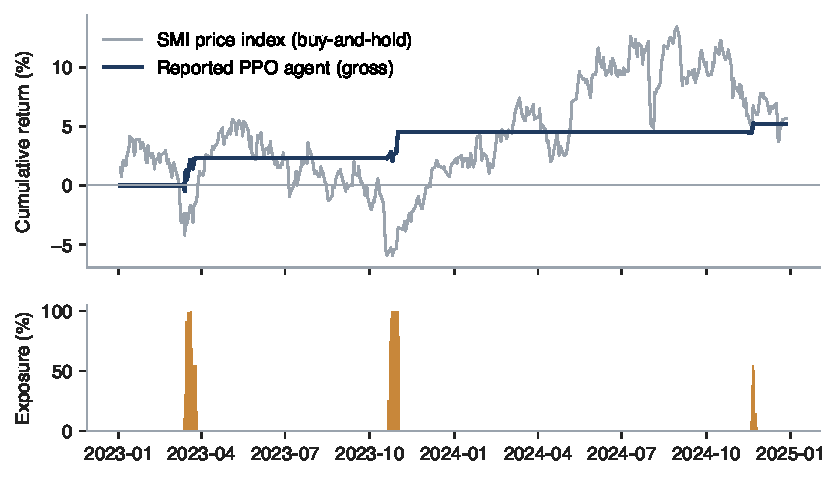
\includegraphics[width=\linewidth]{figs/f1_path.pdf}
\caption{Reported model on the test window: cumulative gross return against the SMI (top) and daily exposure (bottom). Flat segments are days at exactly zero exposure.}
\label{fig:path}
\end{figure}

\subsection{Provenance: what the saved model actually is}\label{sec:provenance}

The thesis states that the reported model was trained for 10,000 timesteps on 2010--2022, with a 2021--2022 validation period, and evaluated out-of-sample on 2023--2024. The saved model contradicts this. Its file records 1,001,472 timesteps (489 rollout-and-update cycles, 156,480 optimiser steps) in a single run, with episodes of 3,725 steps: the length of the full 2010--2024 series. There is no checkpoint and no validation loop. The test years were therefore in its training data, and Table~\ref{tab:reported} is an in-sample result.

This is the most serious error in the thesis and I correct it here. The right question is whether the leak \emph{created} the result. To answer it, I re-trained the same configuration without the test years.

\begin{table}[ht]
\centering\small
\caption{Control C: same configuration as the reported model (1M timesteps), thesis accounting, test window 2023--2024.}
\label{tab:control}
\begin{tabular}{@{}llcccc@{}}
\toprule
\textbf{Training data} & \textbf{Seed} & \textbf{Sharpe} & \textbf{Max DD} & \textbf{Cum.\ return} & \textbf{Days invested} \\
\midrule
2010--2022 (out-of-sample) & 0 & 1.29 & $-0.62\%$ & 4.22\% & 22 \\
 & 1 & 1.25 & $-0.68\%$ & 3.82\% & 15 \\
 & 2 & 1.04 & $-1.08\%$ & 5.35\% & 33 \\
\addlinespace
2010--2024 (in-sample, as reported) & 0 & 1.05 & $-1.04\%$ & 5.39\% & 32 \\
 & 1 & 1.14 & $-0.74\%$ & 4.90\% & 30 \\
 & 2 & 1.25 & $-0.73\%$ & 4.94\% & 23 \\
\midrule
Reported model & -- & 1.17 & $-0.77\%$ & 5.18\% & 27 \\
\bottomrule
\end{tabular}
\end{table}

Trained without the test years, the agent behaves the same way: mostly cash, a Sharpe ratio between 1.0 and 1.3, a drawdown of about 1\% or less, and entries in the same windows (two of the three out-of-sample seeds enter in all three windows of the reported model). The leak did not produce the result. The next sections show what did.

\subsection{Is it timing, or is it cash?}\label{sec:cash}

Figure~\ref{fig:seeds} places every trained agent by its mean exposure and its return. The configuration printed in the thesis (E1, 10,000 timesteps) mostly never invests: 15 of 30 seeds hold exactly zero on every day and two more hold at most 0.11\% on one day. The 13 seeds that do invest have Sharpe ratios of 1.12 to 1.48 but returns of only 0.11\% to 3.16\% over two years. All agents sit in a corner of low exposure, below buy-and-hold and close to cash.

\begin{figure}[ht]
\centering
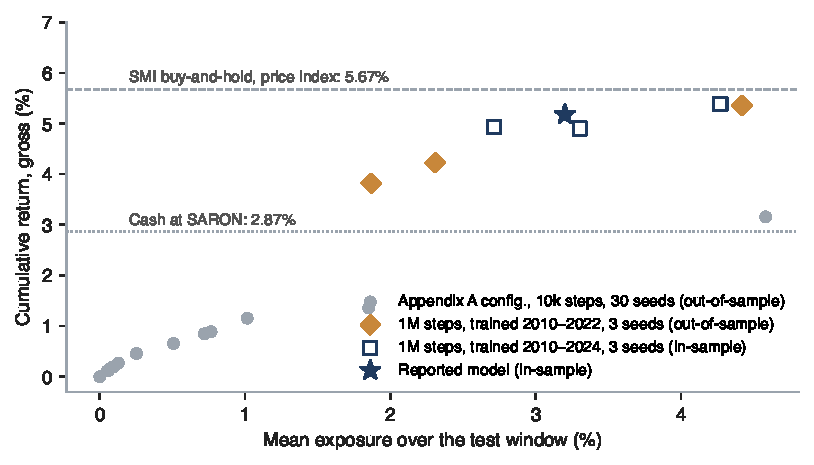
\includegraphics[width=\linewidth]{figs/f3_seeds.pdf}
\caption{Mean exposure against gross cumulative return for every trained agent, test window 2023--2024.}
\label{fig:seeds}
\end{figure}

A Sharpe ratio above 1 at 3\% mean exposure is easy to obtain: holding the index for a handful of days produces a small, positive return with tiny volatility. A constant 10\% exposure with idle cash at SARON already gives a drawdown of only $-0.68\%$. The low drawdown is what the cost specification predicts for an agent that rarely invests; it is not evidence of downside protection learned from the state.

\subsection{A fair comparison}\label{sec:fair}

Thesis accounting is generous to the agent in one way and unfair in another. Its idle cash earns nothing, while real cash earned 2.87\% over the window; and the benchmarks ignore dividends. Under consistent accounting (Figure~\ref{fig:scoreboard}), the reported model returns 7.5\% with a Sharpe ratio over SARON of 1.04. Total-return buy-and-hold returns 14.3\% (Sharpe 0.52) and a real 60/40 portfolio 15.3\% (Sharpe 0.81). The agent's Sharpe ratio is still the highest, but its return is about half that of the real benchmarks, and as the next section shows the Sharpe gap is not statistically significant.

\begin{figure}[ht]
\centering
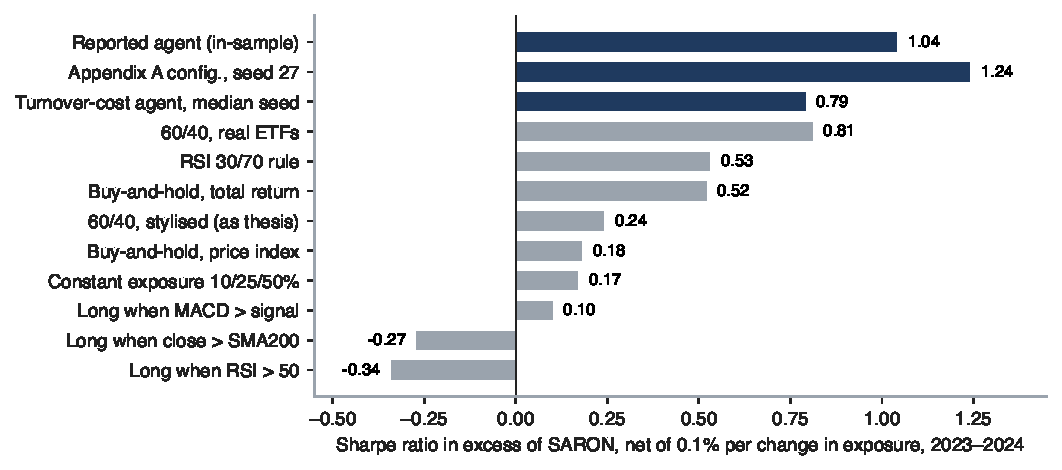
\includegraphics[width=\linewidth]{figs/f2_scoreboard.pdf}
\caption{Consistent accounting, 2023--2024: idle cash earns SARON, every strategy pays 0.1\% per unit change in exposure. Agents in navy, benchmarks and rules in grey.}
\label{fig:scoreboard}
\end{figure}

\begin{table}[ht]
\centering\small
\caption{Consistent accounting, 2023--2024 (selected strategies).}
\label{tab:fair}
\begin{tabular}{@{}lcccc@{}}
\toprule
\textbf{Strategy} & \textbf{Sharpe over SARON} & \textbf{Cum.\ return} & \textbf{Max DD} & \textbf{Volatility} \\
\midrule
Reported model (in-sample) & 1.04 & 7.5\% & $-0.8\%$ & 2.2\% \\
Turnover-cost agent, median seed & 0.79 & 8.1\% & $-2.6\%$ & 3.2\% \\
Buy-and-hold, price index & 0.18 & 5.7\% & $-11.0\%$ & 11.2\% \\
Buy-and-hold, total return & 0.52 & 14.3\% & $-10.5\%$ & 11.6\% \\
60/40, real ETFs & 0.81 & 15.3\% & $-6.6\%$ & 7.5\% \\
RSI 30/70 rule & 0.53 & 11.0\% & $-9.2\%$ & 7.7\% \\
Cash at SARON & 0 & 2.9\% & 0 & 0 \\
\bottomrule
\end{tabular}
\end{table}

\subsection{Formal tests}\label{sec:tests}

Table~\ref{tab:tests} reports the tests of equal Sharpe ratios. None is significant at 5\%, before or after the Holm adjustment. The reported model's Sharpe advantage over buy-and-hold ($+0.87$) has a standard error of 0.76: with 499 days and an agent that is invested on 27 of them, the data cannot distinguish its Sharpe ratio from the index's. Across seeds the picture is the same: none of the 15 testable E1 seeds ($p$ from 0.064 to 0.37) and none of the 10 E2 seeds ($p$ from 0.15 to 0.82) rejects at 5\%.

\begin{table}[ht]
\centering\small
\caption{Tests of equal Sharpe ratios \citep{ledoit2008}: HAC-studentized, circular block bootstrap (block 10, 4,999 resamples), two-sided.}
\label{tab:tests}
\begin{tabular}{@{}llcccc@{}}
\toprule
\textbf{Agent} & \textbf{vs} & \textbf{Diff.} & \textbf{s.e.} & $\boldsymbol{p}$ & \textbf{Holm} \\
\midrule
Reported, thesis accounting & Buy-and-hold, price & $+0.87$ & 0.76 & 0.26 & -- \\
\addlinespace
Reported, consistent & Buy-and-hold, price & $+0.86$ & 0.75 & 0.27 & 0.80 \\
 & Buy-and-hold, total return & $+0.52$ & 0.75 & 0.50 & 1.00 \\
 & 60/40, real ETFs & $+0.22$ & 0.78 & 0.77 & 1.00 \\
\addlinespace
Turnover-cost, median seed & Buy-and-hold, price & $+0.62$ & 0.86 & 0.49 & 1.00 \\
 & Buy-and-hold, total return & $+0.28$ & 0.86 & 0.75 & 1.00 \\
 & 60/40, real ETFs & $-0.02$ & 0.88 & 0.99 & 1.00 \\
 & RSI 30/70 rule & $+0.26$ & 0.85 & 0.76 & 1.00 \\
\bottomrule
\end{tabular}
\end{table}

\subsection{A redesigned agent: cost on trading, not on holding}\label{sec:turnover}

If the holding cost drives the agent into cash, the obvious fix is to charge the cost where it occurs. Agent E2 pays $0.1\%\times|\Delta A_t|$, earns SARON on idle cash inside its reward, and sees a richer state: 1-, 5- and 20-day returns, 20-day volatility, RSI/100, MACD/price and its previous exposure. It was trained with 10 seeds for 200,000 timesteps each.

The redesigned agent does take real exposure: a median of 13\% (5\% to 53\%), invested on 20\% of days, 33 to 104 trades. Its median Sharpe ratio over SARON is 0.75 (0.36 to 1.18) and its median return 8.4\% (4.9\% to 13.1\%). All 10 seeds beat price buy-and-hold on Sharpe, 7 beat total-return buy-and-hold and the RSI rule, and 4 beat the real 60/40. None of these differences is significant (Table~\ref{tab:tests}), and the edge depends on cheap trading: at 0.25\% per unit of exposure changed, the median seed's Sharpe falls to 0.12 (Figure~\ref{fig:cost}). For reference, a Swiss retail trade costs about 0.1\% in commission plus 0.075\% stamp duty.

\begin{figure}[ht]
\centering
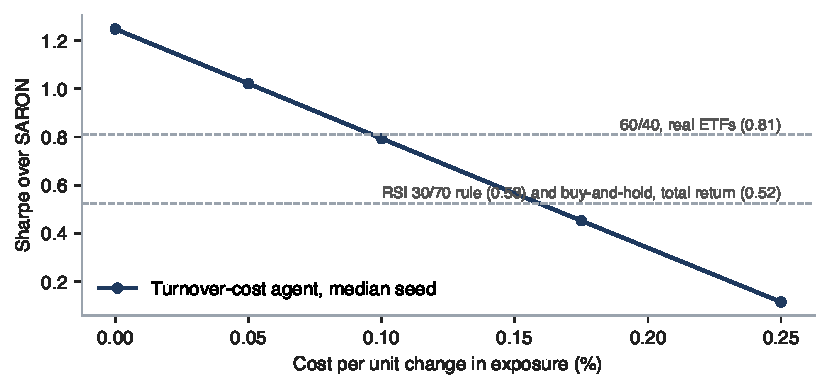
\includegraphics[width=\linewidth]{figs/f4_cost.pdf}
\caption{Turnover-cost agent (median seed): Sharpe over SARON when its actions are charged different trading costs.}
\label{fig:cost}
\end{figure}

\subsection{Stress windows}\label{sec:stress}

The thesis claimed downside protection. The test window had no crash, so I trained walk-forward agents and evaluated them on 2020 (COVID crash) and 2022 (rate shock). The right comparison for an agent with low average exposure is a constant exposure at the same level: if the agent has learned to de-risk, it should draw down less than that constant.

\begin{figure}[ht]
\centering
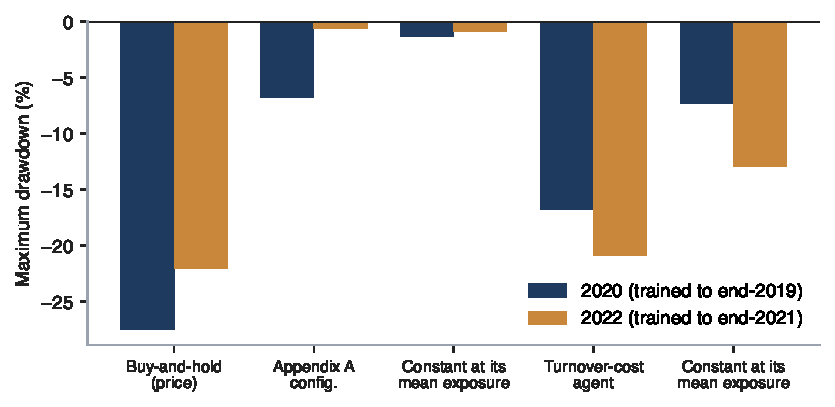
\includegraphics[width=\linewidth]{figs/f5_stress.pdf}
\caption{Maximum drawdown in two stress windows (medians across seeds), against a constant exposure equal to each agent's own mean exposure.}
\label{fig:stress}
\end{figure}

It does not (Figure~\ref{fig:stress}). In 2020 both agents drew down more than their constant-exposure twin ($-6.8\%$ vs $-1.3\%$; $-16.8\%$ vs $-7.3\%$), and in 2022 the turnover-cost agent did too ($-20.9\%$ vs $-12.9\%$). The original configuration's small drawdown in 2022 ($-0.65\%$) is in line with a constant 2\% exposure ($-0.9\%$). There is no sign of learned de-risking: the protection comes from not being invested.

% ------------------------------------------------------------------ 6
\section{Discussion}\label{sec:discussion}

\paragraph{Closing the hypotheses}
\textbf{H1} is met only as a point estimate. The agent's Sharpe ratio is higher than buy-and-hold's in every specification, but the difference is never significant, and under consistent accounting it earns about half the return of the real benchmarks. \textbf{H2} is met mechanically: the drawdown is smaller because the agent is almost never invested, and in stress windows it does no better than a constant exposure at its own average level. Neither hypothesis supports the claim that the agent learned to time the market.

\paragraph{What the result is}
The headline result is real in the sense that it reproduces, and it survives removing the test years from training. But it is explained by two design choices, not by learning: a cost that makes cash the best default action, and an accounting that compares a near-cash strategy with benchmarks stripped of dividends and with cash that earns nothing. Once both are fixed, the agent is a low-risk, low-return strategy whose edge cannot be told apart from noise.

\paragraph{A checklist for DRL back-tests}
The audit suggests six checks that would have caught each problem before submission:
\begin{enumerate}[leftmargin=1.4em]
  \item \textbf{Provenance.} Read the saved model's training metadata (timesteps, episode length) and confirm it matches the protocol.
  \item \textbf{Exposure first.} Report mean exposure and days invested next to every Sharpe ratio.
  \item \textbf{Cost where it occurs.} Charge trading costs on changes in position; compare any cost with the asset's mean return.
  \item \textbf{Same accounting for everyone.} Idle cash at the risk-free rate, total-return benchmarks, the same costs.
  \item \textbf{Many seeds and a formal test.} Report the distribution across seeds and a studentized test of equal Sharpe ratios.
  \item \textbf{Matched controls.} Compare with a constant exposure at the agent's own mean exposure, and with simple rules.
\end{enumerate}

% ------------------------------------------------------------------ 7
\section{Limitations and future work}

The test window has 499 days, which gives little power: even a true Sharpe difference of about 0.9 would usually not be detected. The control uses three seeds per arm. The SARON series is a proxy built from the SNB policy rate. Static benchmarks are rebalanced daily without cost (with cost, the real 60/40 gives Sharpe 0.80 and 15.0\%). Taxes and the bid--ask spread are not modelled.

The natural next step is a genuine allocation problem: an agent that sets weights over four or five ETFs (equities, Swiss equities, bonds, gold, cash), with a cost on turnover, cash at the risk-free rate, walk-forward training over several windows, at least 10 seeds, a protocol fixed before seeing results, and benchmarks such as 60/40, equal weight, risk parity \citep{maillard2010} and volatility targeting.

% ------------------------------------------------------------------ 8
\section{Conclusion}

A PPO agent on the SMI produced a Sharpe ratio four times that of the index with almost no drawdown. On audit, the reported model turned out to have been trained on its test years; trained without them, it behaves the same, so the leak was not the cause. The cause is a daily holding cost five times the index's mean daily return, which teaches the agent to stay in cash, together with an accounting that flatters a near-cash strategy. Under fair accounting the agent earns about half of what a real 60/40 portfolio earned, no Sharpe-ratio difference is significant, a redesigned agent's edge disappears at realistic trading costs, and no agent de-risked in a crash. The lesson is less about reinforcement learning than about evaluation: a DRL back-test should be read through its exposure, its costs and its accounting before its Sharpe ratio.

\section*{Reproducibility}
\addcontentsline{toc}{section}{Reproducibility}
\small
All numbers in this edition come from scripts and result files kept with the project: re-evaluation of the saved model (\texttt{avaliar\_modelo\_original.py}, \texttt{results/original\_model\_v2\_eval.json}, \texttt{results/original\_model\_v2\_test\_path.csv}); tests on it (\texttt{stats\_saved\_model.py}); the control (\texttt{controlo\_1M.py}, \texttt{results/E4\_control\_1M.json}); experiments E1--E3 and benchmarks (\texttt{experiments.py}, \texttt{results/}); tests (\texttt{stats\_tests.py}); and the figures of this edition (\texttt{portfolio/make\_figs.py}). Independent re-verification scripts are in \texttt{verificacao-2026-10-18/}. The thesis's own implementation is printed in its Appendix~A.

\section*{Use of AI tools}
\addcontentsline{toc}{section}{Use of AI tools}
Generative AI (Claude, Gemini) was used for coding support, grammar and revision of the prose, and, after submission, for help with the audit scripts and the layout of this edition. All analyses were run and checked by the author.
\normalsize

% ------------------------------------------------------------------ refs
\begin{thebibliography}{99}\small
\setlength{\itemsep}{0.15em}
\bibitem[Appel(2005)]{appel2005} Appel, G. (2005). \emph{Technical analysis: Power tools for active investors}. FT Prentice Hall.
\bibitem[Bailey et~al.(2017)]{bailey2017} Bailey, D.~H., Borwein, J.~M., López de Prado, M., \& Zhu, Q.~J. (2017). The probability of backtest overfitting. \emph{Journal of Computational Finance}, 20(4), 39--69.
\bibitem[Black and Litterman(1992)]{black1992} Black, F., \& Litterman, R. (1992). Global portfolio optimization. \emph{Financial Analysts Journal}, 48(5), 28--43.
\bibitem[Garrido-Merchán et~al.(2023)]{garrido2023} Garrido-Merchán, E.~C., Mora-Figueroa-Cruz-Guzmán, S., \& Coronado-Vaca, M. (2023). Deep reinforcement learning for ESG financial portfolio management. arXiv:2307.09631.
\bibitem[Gort et~al.(2022)]{gort2022} Gort, B.~J.~D., Liu, X.-Y., Sun, X., Gao, J., Chen, S., \& Wang, C.~D. (2022). Deep reinforcement learning for cryptocurrency trading: Practical approach to address backtest overfitting. arXiv:2209.05559.
\bibitem[Hieu(2020)]{hieu2020} Hieu, L.~T. (2020). Deep reinforcement learning for stock portfolio optimization. arXiv:2012.06325.
\bibitem[Hirsa et~al.(2021)]{hirsa2021} Hirsa, A., Osterrieder, J., Hadji-Misheva, B., \& Posth, J.-A. (2021). Deep reinforcement learning on a multi-asset environment for trading. arXiv:2106.08437.
\bibitem[Holm(1979)]{holm1979} Holm, S. (1979). A simple sequentially rejective multiple test procedure. \emph{Scandinavian Journal of Statistics}, 6(2), 65--70.
\bibitem[Jiang et~al.(2017)]{jiang2017} Jiang, Z., Xu, D., \& Liang, J. (2017). A deep reinforcement learning framework for the financial portfolio management problem. arXiv:1706.10059.
\bibitem[Ledoit and Wolf(2004)]{ledoit2004} Ledoit, O., \& Wolf, M. (2004). Honey, I shrunk the sample covariance matrix. \emph{The Journal of Portfolio Management}, 30(4), 110--119.
\bibitem[Ledoit and Wolf(2008)]{ledoit2008} Ledoit, O., \& Wolf, M. (2008). Robust performance hypothesis testing with the Sharpe ratio. \emph{Journal of Empirical Finance}, 15(5), 850--859.
\bibitem[López de Prado(2018)]{lopezdeprado2018} López de Prado, M. (2018). \emph{Advances in financial machine learning}. Wiley.
\bibitem[Maillard et~al.(2010)]{maillard2010} Maillard, S., Roncalli, T., \& Teiletche, J. (2010). The properties of equally weighted risk contribution portfolios. \emph{The Journal of Portfolio Management}, 36(4), 60--70.
\bibitem[Mandelbrot(1963)]{mandelbrot1963} Mandelbrot, B. (1963). The variation of certain speculative prices. \emph{The Journal of Business}, 36(4), 394--419.
\bibitem[Markowitz(1952)]{markowitz1952} Markowitz, H. (1952). Portfolio selection. \emph{The Journal of Finance}, 7(1), 77--91.
\bibitem[Michaud(1989)]{michaud1989} Michaud, R.~O. (1989). The Markowitz optimization enigma: Is `optimized' optimal? \emph{Financial Analysts Journal}, 45(1), 31--42.
\bibitem[Newey and West(1987)]{newey1987} Newey, W.~K., \& West, K.~D. (1987). A simple, positive semi-definite, heteroskedasticity and autocorrelation consistent covariance matrix. \emph{Econometrica}, 55(3), 703--708.
\bibitem[Politis and Romano(1992)]{politis1992} Politis, D.~N., \& Romano, J.~P. (1992). A circular block-resampling procedure for stationary data. In R.~LePage \& L.~Billard (Eds.), \emph{Exploring the limits of bootstrap} (pp.~263--270). Wiley.
\bibitem[Raffin et~al.(2021)]{raffin2021} Raffin, A., Hill, A., Gleave, A., Kanervisto, A., Ernestus, M., \& Dormann, N. (2021). Stable-Baselines3: Reliable reinforcement learning implementations. \emph{Journal of Machine Learning Research}, 22(268), 1--8.
\bibitem[Schulman et~al.(2017)]{schulman2017} Schulman, J., Wolski, F., Dhariwal, P., Radford, A., \& Klimov, O. (2017). Proximal policy optimization algorithms. arXiv:1707.06347.
\bibitem[Sharpe(1966)]{sharpe1966} Sharpe, W.~F. (1966). Mutual fund performance. \emph{The Journal of Business}, 39(1), 119--138.
\bibitem[Sharpe(1994)]{sharpe1994} Sharpe, W.~F. (1994). The Sharpe ratio. \emph{The Journal of Portfolio Management}, 21(1), 49--58.
\bibitem[Wilder(1978)]{wilder1978} Wilder, J.~W., Jr. (1978). \emph{New concepts in technical trading systems}. Trend Research.
\bibitem[Wu and Hargreaves(2024)]{wu2024} Wu, W., \& Hargreaves, C.~A. (2024). Deep reinforcement learning approach to portfolio optimization in the Australian stock market. \emph{AI, Computer Science and Robotics Technology}, 3(1), 1--31.
\bibitem[Xiong et~al.(2018)]{xiong2018} Xiong, Z., Liu, X.-Y., Zhong, S., Yang, H., \& Walid, A. (2018). Practical deep reinforcement learning approach for stock trading. arXiv:1811.07522.
\bibitem[Yang et~al.(2020)]{yang2020} Yang, H., Liu, X.-Y., Zhong, S., \& Walid, A. (2020). Deep reinforcement learning for automated stock trading: An ensemble strategy. In \emph{Proceedings of the First ACM International Conference on AI in Finance (ICAIF '20)}. ACM.
\end{thebibliography}

\end{document}
